\section{Анализ электронных писем корпорации Enron}

\subsection{Длины писем}

Аналогично тому, как было сделано для набора Клинтон, можно проанализировать распределение длин
писем (по количеству слов). 
Гистограмма, как и в случае писем Клинтон, соответствует интуитивным ожиданиям -- более длинные письма пишутся реже:

\begin{figure}[H]
\centering
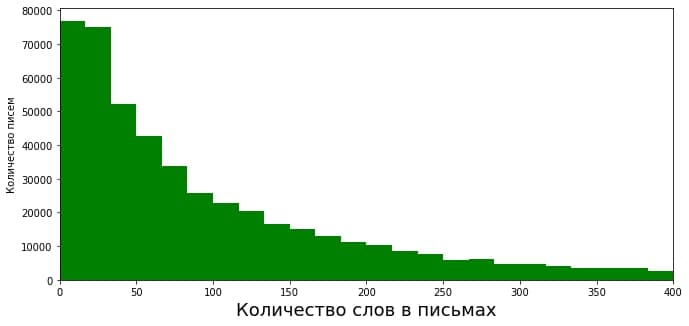
\includegraphics[scale=0.75]{pics/enron_emails_words_count.jpg}
\caption{Распределение количества слов в письмах в наборе $Enron$}
\end{figure}



\subsection{Время отправки писем}

\begin{itemize}

\item Как и наборе Клинтон, в метаданных писем содержится информация об дате отправки писем,
поэтому можно проанализировать различную полезную информацию, например в какие года
были отправлены письма:

\begin{figure}[H]
\centering
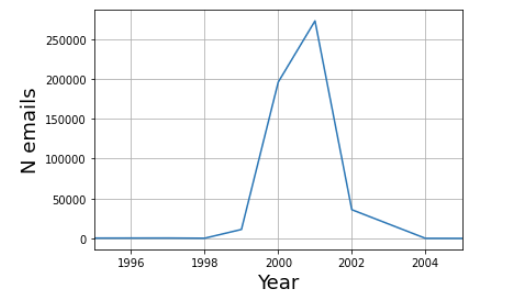
\includegraphics[scale=0.7]{pics/enron_year.png}
\caption{График количества отправленных писем по годам в наборе $Enron$}
\end{figure}

График соответствует наибольшей активности компании в 2000-2001 годах и банкротству к концу 2001 года.

\item Аналогично можно проанализировать дни недели отправки писем:

\begin{figure}[H]
\centering
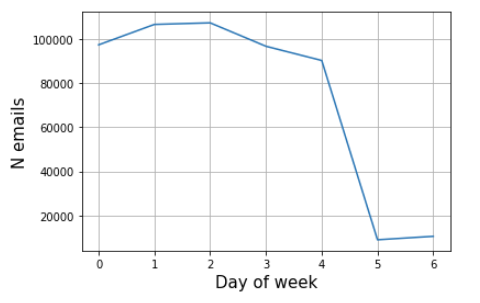
\includegraphics[scale=0.7]{pics/enron_week.png}
\caption{График количества отправленных писем по дням недели в наборе $Enron$}
\end{figure}


Этот график также выглядит естественно --- наибольшее число писем во вторник и среду, в середине рабочей недели, наименьшее --- в выходные дни.

\item В отличие от набора Клинтон, в наборе $Enron$ дополнительно содержится информация о том,
в какое время суток было отправлено письмо:


\begin{figure}[H]
\centering
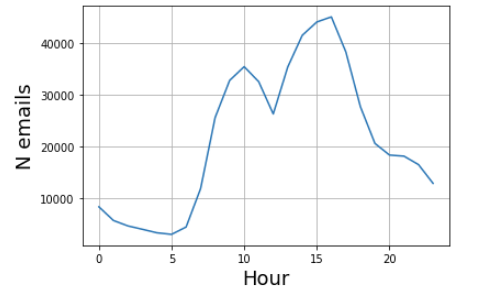
\includegraphics[scale=0.7]{pics/enron_hour.png}
\caption{График количества отправленных писем по времени суток в наборе $Enron$}
\end{figure}

На графике вышем видим наибольшую продуктивность во вторую половину дня, низкую активность в ночные часы, а также аномалию в самом разгаре дня, объсняющуюся обеденным перерывом.

\end{itemize}

\subsection{Частотность слов}

Для интерпретации самых часто используемых слов использовались так называемые облака слов.

Облако слов --- это метод визуализации данных, используемый для представления текстовых данных, в которых размер каждого слова указывает его частоту или важность. Важные точки текстовых данных могут быть выделены с помощью облака слов. Облака слов широко используются для анализа данных с веб-сайтов социальных сетей.


\begin{itemize}
\item В нашем случае можно, например, построить облако слов, используя информацию о темах писем:

\begin{figure}[H]
\centering
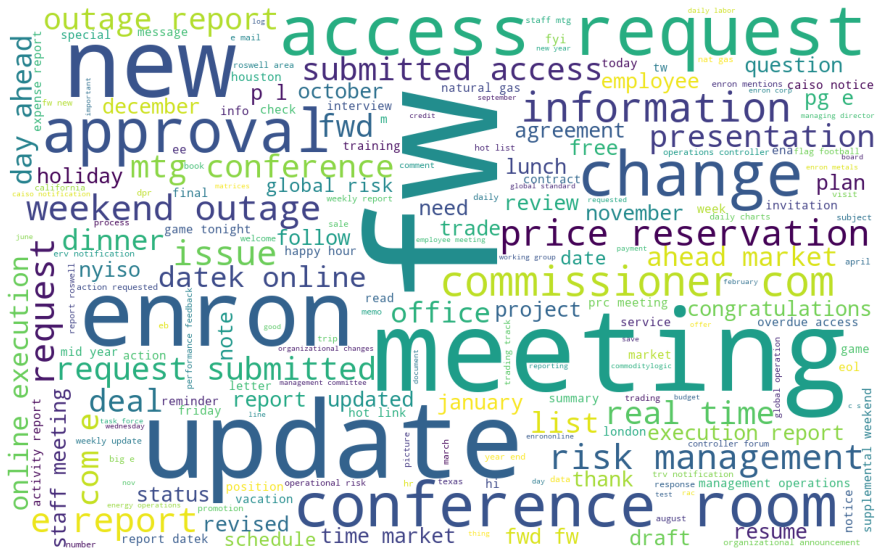
\includegraphics[scale=0.6]{pics/enron_wordcloud_subject.png}
\caption{Облако слов по словам из названий тем писем в наборе $Enron$}
\end{figure}



Слова, встречающиеся в темах писем: \texttt{meeting}, \texttt{conference room}, \texttt{update}, \texttt{approval},\texttt{access request}, \texttt{enron}.

\item Аналогично можно построить облако слов по информации из содержаний писем:

\begin{figure}[H]
\centering

\includegraphics[scale=0.6]{pics/enron_wordcloud_content.png}
\caption{Облако слов по словам из содержаний писем в наборе $Enron$}
\end{figure}


Слова, встречающиеся в содержании писем: \texttt{enron}, \texttt{week}, \texttt{thank}, \texttt{know}, \texttt{new}.

\end{itemize}

\subsection{Отправители и получатели писем}

\begin{itemize}


\item На основании отправителей и получателей писем можно посчитать некоторую интересную статистику. Например, можно найти 20 адресов, с которых было отправлено наибольшее количество электронных писем:


\begin{figure}[H]
\centering
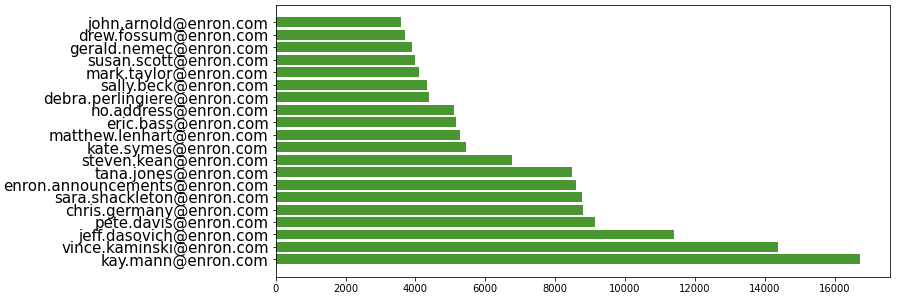
\includegraphics[scale=0.5]{pics/enron_most_sent.png}
\caption{Распределений количества писем по 20 адресам, с которых было отправлено наибольшее количество электронных писем в наборе $Enron$}
\end{figure}


\item Аналогично, можно найти 20 адресов, на которые было отправлено наибольшее количество электронных писем:


\begin{figure}[H]
\centering
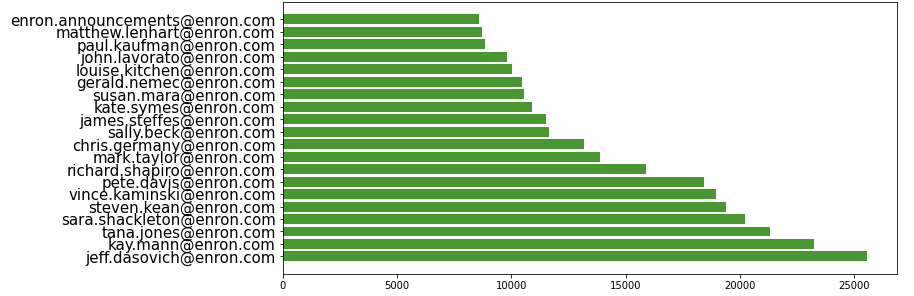
\includegraphics[scale=0.5]{pics/enron_most_recieved.png}
\caption{Распределений количества писем по 20 адресам, на которые было отправлено наибольшее количество электронных писем в наборе $Enron$}
\end{figure}


Как видим, в графиках распределения получателей и отправителей писем много различий --- некоторые люди пишут писем меньше, чем получают и наоборот.

\item Теперь посмотрим количество писем между фиксированной парой собеседников. Рассмотрим только электронные письма, отправленные на один адрес электронной почты, так как они могут быть более важными личными сообщениями.

\begin{table}[H]
\centering
\begin{tabular}{ | l | l | l | }
\hline
Отправитель & Получатель & Количество \\ \hline
pete.davis & pete.davis & 9141 \\ \hline
vince.kaminski & vkaminski@aol.com & 4308 \\ \hline
enron.announcements & all.worldwide & 2206 \\ \hline
enron.announcements & all.houston & 1701 \\ \hline
kay.mann & suzanne.adams & 1528 \\ \hline
vince.kaminski & shirley.crenshaw & 1190 \\ \hline
steven.kean & maureen.mcvicker & 1014 \\ \hline
kay.mann & nmann@erac.com	 & 980 \\ \hline
kate.symes & evelyn.metoyer & 	915 \\ \hline
kate.symes & kerri.thompson	 & 859 \\ \hline
\end{tabular}
\caption{Таблица количества писем по парам собеседников в наборе $Enron$}
\end{table}

Здесь интересно, что некоторые люди отправляют сами себе много электронных писем.


\end{itemize}
